Throughout this paper, bold capital letters denote matrices (e.g., $\mathbf{X}$) and bold lower-case letters denote column vectors (e.g., $\mathbf{x}$). $\norm{\mathbf{X}}_2 =
(\mathbf{X}^T\mathbf{X})^{1/2}$ and $\norm{\mathbf{X}}_1 = \sum_i |\mathbf{x}_i|$
denote the $l_2$ and $l_1$ norms, respectively, with $T$ indicating the
matrix transpose. We also denote $\norm{\mathbf{X}}_F =
(\text{Tr}(\mathbf{X}^T\mathbf{X}))^{1/2}$ as the Frobenius norm, where
Tr indicate the trace of a matrix, i.e.,  $\text{Tr}(X)\equiv \sum_{i=1}^n \mathbf{x}_{ii}$.

This section contains the theory to implement a model such as the model presented in section \ref{sec:fab}. We first present a brief overview of the mathematical background behind Optimization, Machine Learning and Artificial Neural Networks (ANN) in sections \ref{sec:opt},\ref{sec:ml} and \ref{sec:ann} respectively. This theory leads up to all the necessary details involved with Sparse Coding, which is presented in \ref{sec:sc} with two examples in computer vision and speech recognition to give the reader a better understanding of the concept. We later present an underlying concept called Non-Negative Matrix-Factorization in section \ref{sec:nnsc} and the proof behind it. This technique is commonly used when dealing with tasks involving only positive values. 

%Lastly we present techniques for sparse approximations in section \ref{sec:regularization}.

\label{sec:theoretical}

\subsection{Optimization}
\label{sec:opt}
A problem that consists of finding the best solution from a set of feasible solutions. In mathematics and computer science, we refer this as a optimization problem. The standard form of a optimization problem is defined as

\begin{align*}
& \underbrace{\text{min}}_{x} \qquad f(x) \\
& \text{subject to} \quad g_i(x) \leq 0, \ i = 0,\dots,n
\end{align*}
where we define $f(x)$ as the objective function to be minimized with respect to $x$ and $g_i(x)$ as the $i$:th constraint. By convention, the standard form is to minimize the objective function, we can maximize by negating the expression above \cite{convex}.

\subsubsection{Cost function}

An objective function that is of standard form is often referred to as a cost or loss function that maps events or values of variables to some value that represents the "cost" involving that particular event. In classification, the cost is usually portrayed as "penalty" involving an incorrect classification. 

Supervised learning tasks, described in \ref{sec:ml}, such as regression or classification for parameter estimation can be formulated as a loss function over a training set. The goal is to find the models that represent the input well; and the loss function quantifies the amount of deviation of the prediction from the true values \cite{convex}.

\subsection{Machine Learning}
\label{sec:ml}
Machine learning can be considered a sub-field of computer science and statistics which can be described as the study of algorithms that can learn from data. Mostly Machine learning is employed on computational tasks where designing and programming explicit, rule-based algorithms is infeasible. The common applications include spam filtering, optical character recognition (OCR), search engines and computer vision. It also has ties to both artificial intelligence and optimization.

Machine learning tasks are typically classified into three broad categories, depending on the nature of the learning "signal" or "feedback" available to a learning system. One category is Supervised learning; where the computer is presented with example inputs and their desired outputs, given by the user, and the goal is to learn a general rule that maps inputs to outputs. The second category is Unsupervised learning, where no labels are given to the learning algorithm. This way the algorithm has to find its own structure in the input, this algorithm can be run to do stand-alone unsupervised learning (discover hidden patterns) or a means towards another type of end. Sparse Coding, which forms the basis of this thesis is a neural network model for unsupervised learning. Lastly we have reinforcement learning where a computer program interacts with a dynamic environment in which it must perform a certain goal (such as driving a vehicle), without a teacher explicitly telling it whether it has come close to its goal or not. Another example is learning to play a game by playing against an opponent \cite{ainorvig}.

A core objective of a learner is to generalize from its experience. Generalization in this context is the ability of a learning machine to perform accurately on new, unseen examples/tasks after having experienced a learning data set \cite{bishop, bengio}. The training examples usually come from some unknown probability distribution and the learner has to build a general model so as to produce sufficiently accurate predictions from incoming new examples. 

In machine learning one can simplify the inputs by mapping them into a lower-dimensional space through dimensionality reduction, described in section \ref{sec:dim}.

\subsubsection{Dimensionalty Reduction}
\label{sec:dim}

Representing an object as a vector of $n$ elements, we say that the vector is in $n$-dimensional space. Dimensionalty reduction refers to a process of representing the object of $n$-dimensional vector to an $m$-dimensional vector, where $m < n$. By refining the data in this way, we may lose information that might be valuable but we can represent it using less dimensions and in some cases we can even make a better prediction or analysis using this subspace. The common linear dimensionality reduction is called Principal Component Analysis (PCA), which find "internal axes" of a dataset, called components and sort by importance. It performs a linear mapping of the data to a lower-dimensional space in such a way that the variance of the data in the low-dimensional representation is maximized. The original space is not retained, i.e. we have lost some information but keep the most important variance to the space spanned by a few eigenvectors. The first $m$ components are then used as the new basis. Each of these components may be thought of as a high-level feature, describing data vectors better than original axes \cite{dr}.

Dimensionality reduction can be divided into feature selection and feature extraction. Feature selection approaches try to find a subset of the original variables, while feature extraction transforms the data in high-dimensional space to that of a fewer dimensional space. The data transformation may be linear, as in PCA, but many nonlinear dimensionality reduction techniques also exist \cite{samet}. 

A different approach to nonlinear dimensionality reduction is through the use of autoencoders, a special kind of feed-forward neural networks with a bottle-neck hidden layer, which is presented in-depth in section \ref{sec:autoencoders}.

\subsubsection{Deep Learning}
\label{sec:deeplearning}

A branch of machine learning based on algorithms that try to model high-level abstractions in data by using complex structures or multiple non-linear transformations is referred to deep learning \cite{deep, deep2}. Deep learning focuses on learning representations of data, where it has maybe come to replacing handcrafted features with efficient algorithms for unsupervised or semi-supervised feature learning and hierarchical feature extraction \cite{deep3}.

Some representation are based on interpreting information processsing in a nervous system inspired by advances in neuroscience, such as neural coding which attempts to define a relationship between the stimulus and the neuronal responses and the relationship among the electrical activity of the neurons in the brain \cite{nervous}, see section \ref{sec:scnn} for more information.



\subsection{Artificial Neural Networks}
\label{sec:ann}

In machine learning, a family of statistical learning algorithms called artificial neural networks (ANN) that were inspired by the work of McCulloch, Warren; Walter Pitts as early as 1943 to reflect a central nervous systems of animals \cite{1943}. Generally ANN is a network with connected nodes and edges that form a artificial "biological neural network" which compute values from inputs provided by the edges connected to the nodes, even though the relation between the model and the brain is debated to what degree it really represents the brain \cite{brain}. 

ANN models are essentially mathematical functions defining a function 
\begin{equation} 
f : X \rightarrow Y
\end{equation}

but sometimes models are also associated with a particular learning algorithm, like the perceptron presented in the section \ref{sec:perceptron} below. The learning output is obtained by connection weights, parameters and specific architecture by the learning algorithm. Two frameworks where ANN have made a great contribution is computer vision and speech recognition tasks, where rule-based programming have been unsuccessful at detecting patterns \cite{perceptron}. The connection between neural networks and Sparse Coding is explained in section \ref{sec:scnn}.

There are two main ways to "feed" the network with information. One being that of a feedforward neural network, the term “feedforward” indicates that the network has links that extend in only one direction. Except during training, there are no backward links in a feedforward network; all links proceed from input nodes toward output nodes. Eventually, despite the apprehensions of earlier workers, a powerful algorithm for apportioning error responsibility through a multi-layer network was formulated in the form of the backpropagation algorithm \cite{backpro}. The effects of error in the output nodes are propagated backward through the network after each training case. The essential idea of backpropagation is to combine a non-linear multi-layer perceptron-like system capable of making decisions with the objective error function of the Delta Rule \cite{backpro}.
% checked

\pagebreak
\subsubsection{Perceptron}
\label{sec:perceptron}
The basic concept of a single layer perceptron was introduced by Rosenblatt in 1958 \cite{perceptron}. It computes a single output by forming a linear combination of real-valued inputs and weights to possibly giving it through some non-linear function. This can be written as

\begin{equation} 
 y = \phi( \sum\limits_{i=1}^n a_i x_i + b ) = \phi( \mathbf{a}^T \mathbf{x}+ b )
\end{equation}

where  $\mathbf{a}$ denotes the vector of weights,  $ \mathbf{x}$ is the vector of inputs, $ b$ is the bias and $ \phi$ is the activation function. Usually in multilayer networks, the activation function is often chosen to be the logistic sigmoid $ 1 / (1 + e^{-x})$ or the hyperbolic tangent $ \tanh(x)$. They are convenient as they are close to linear near the origin, while they converge to a value when leaving the origin. This allows perceptron networks to model well both strongly and mildly nonlinear mappings \cite{nonlinear}. Perceptrons were a popular machine learning solution in the 1980s, but since the 1990s faced strong competition from the much simpler support vector machines \cite{svm}. More recently, there has been some renewed interest in backpropagation networks, such as perceptrons due to the successes of deep learning, see section \ref{sec:deeplearning} for more detail.

A typical perceptron layer network consists of source nodes forming the first layer. Following with one or more hidden layers, and an output layer of nodes, in the case where we have three or more layers it is usually called a multilayer perceptron (MLP). The input signal propagates through the network layer-by-layer. The signal-flow of such a network with one hidden layer can be seen in figure \ref{fig:autoencoder} in section \ref{sec:autoencoders}.

The computations performed by such a feedforward network with a single hidden layer with nonlinear activation functions and a linear output layer can be written mathematically as

\begin{equation}
\mathbf{y}= \mathbf{f}(\mathbf{x}) = \mathbf{B}\boldsymbol{\phi}( \mathbf{A}\mathbf{x}+ \mathbf{a} ) + \mathbf{b}
\label{eq:nonlinear}
\end{equation}

where  $\mathbf{x}$ is a vector of inputs and  $\mathbf{y}$ a vector of outputs.  $ \mathbf{A}$ is the matrix of weights of the first layer,  $ \mathbf{a}$ is the bias vector of the first layer.  $ \mathbf{B}$ and  $ \mathbf{b}$ are, respectively, the weight matrix and the bias vector of the second layer. 

MLP networks are typically used in supervised learning problems. Here the training set of input-output is pairs and the network must learn to model the dependency between them. The training here means adapting all the weights and biases ( $ \mathbf{A},
\mathbf{B}, \mathbf{a}$ and  $ \mathbf{b}$ in equation \ref{eq:nonlinear} to their optimal values for the given pairs  $ (\mathbf{x}(t), \mathbf{y}(t))$. The criterion to be optimised is typically the squared reconstruction error.
%to read more on regression see section \ref{sec:regularization}

\begin{equation}
\label{eq:error}
\sum_t \vert\vert\mathbf{f}(\mathbf{x}(t)) - \mathbf{y}(t)\vert\vert^2.
\end{equation}

By setting the same values for the inputs as well as the outputs of the network, MLP networks can be used for unsupervised learning. The values of the hidden neurons extract the sources, this approach however is rather computationally intensive. \cite{hidden}

\subsubsection{Autoencoder}
\label{sec:autoencoders}

Autoencoder is a simple 3-layer neural network where output units (Layer $L_3$) are directly connected back to input units (Layer $L_1$). E.g. in a network presented in the figure below:

\begin{figure}[H]
	\centering
	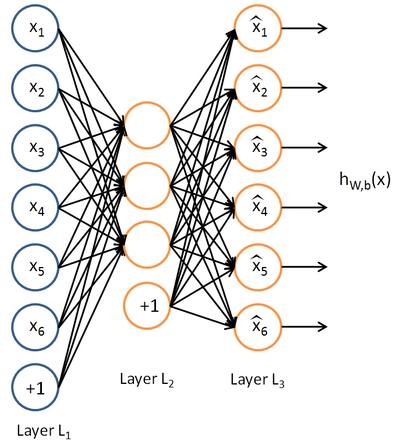
\includegraphics[scale=0.3]{./figures/autoencoder}
	\caption[Caption for LOF]{As a concrete example, suppose the inputs $x$ are the pixel intensity values from a $10 \times 10$ image (100 pixels) so  $n=100$, and there are $s_2=50$ hidden units in layer $L_2$.	\protect\footnotemark}
	\label{fig:autoencoder}
\end{figure}
\footnotetext{Stanford, \texttt{http://ufldl.stanford.edu/wiki/index.php/Autoencoders\_and\_Sparsity},7 April 2013, (accesed 10 July 2015)}
Typically in an autoencoder, the number of hidden units are much less than number of input and output. As a result, it first compresses (encodes) the input vector to "fit" in a smaller representation, and then tries to reconstruct (decode) it back. Here is where Sparse Coding can be said to be an extension of autoencoders with the constraint that the hidden layer must mostly be unused nodes (sparse), for more information on their similarities see the end of section \ref{sec:sc}. Autoencoders simple form can be written as
%\[ D(d(e(x;\theta^r); \theta^d), x) \]

\begin{equation}
\label{eq:auto}
\norm{\mathbf{A}\sigma(\mathbf{A}^T \mathbf{x}) - \mathbf{x}}^2
\end{equation}

where $\sigma$ is a nonlinear function such as the logistic sigmoid, and $\mathbf{A}$ is the activation density of the nodes. Once a deep network is pretrained, input vectors are transformed to a better representation. \cite{autoencoder2}

\subsubsection{Sparse Coding and the connection to Neural Networks}
\label{sec:scnn}

Information retrieved is presented in the brain by the pattern of activations of the nerual connections formed, which we say form a neural code. This defines the pattern at which the neural activity corresponds to each presented information. 
% - rewrite
One property of the neural code is the fraction at which the neurons are active at any time. If a set of $N$ neurons, which can be active in the region $\in [0,1/2]$ corresponding to low activity to strong activity, the expected value of this fraction is the density of the code. If the average fraction is above 1/2 we can replace each active neuron with an inactive one causing the fraction activity to get below 1/2 without loss of information and vice versa. Sparse coding is a neural code, which is of a relatively small set of neurons but with strong activity. For each set of information, a different subset is triggered of all available neurons.\cite{scprimate}

\subsubsection{Local Codes}
Low activity of neurons are local codes, where an item is represented by a small set of neurons or a separate neuron, this way one can ensure that there is no overlap between the representations of two items. To understand this we make an analogy that envolves the characters on a computer keyboard, where each key encodes a single character. This scheme has the advantage that it is simple and is also easy to decode, due to local codes only representing a finite number of combinations. More generalization is essential and a widely observed behavior. \cite{mclaren}

\subsubsection{Dense Distributed Codes}

% - rewrite
The opposite of local codes are dense codes, where the average activity ratio is $\geq 0.5$, the item is represented by activities of all the neurons, which implies a representational capacity of $2^N$. Given the billions of neurons in a human brain, $2^N$, as the number of neurons the representational capacity of a dense code in the brain is immense, therefore its greatest feature is dealing with redundancy. Dense codes limit the number of memories that can be stored in an associative memory by simple learning rules. On the contrast, dense codes may facilitate good generalization performance and high redundancy.

\subsubsection{Sparse Codes}
% - rewrite

These neural codes come to a favorable compromise between dense and local codes by having a small average activity ratio, called sparse codes \cite{scprimate}. We can redeem the capacity of local codes by a modest fraction of active units per pattern, thus interference by items represented simultaneously will be less likely as capacity grows exponentially with average activity ratio. It is more likely that a single layer network with a sparse representation as input can learn to generate a target output \cite{willshaw}. Due to linear discriminant functions being able to map higher proportions, see Perceptrons for linear separability in section \ref{sec:perceptron}. Single layer networks for learning is therefore simpler, faster and substantially more plausible as a way of a biological implementation in the brain, as the redundancy for fault tolerance can be chosen by controlling the sparseness.

For learning various tasks a neural code can therefore contain codewords of varying sparseness. This implies that we want to maximize sparseness while having a high representational capacity. One plausible way would be to assign sparse codes for items of high probability while having distributed codes for lower probability items.
A code with a given average sparseness can contain codewords of varying sparseness. If the goal is to maximize sparseness while keeping representational capacity high, a sensible strategy is to assign sparse codewords to high probability items and more distributed codewords to lower probability items. However, if we would only store identities of active units, the code would have short average discription length \cite{cover}. Some perceptual learning could be explained by prediction of the sparseness of the encoded items with high probability.

Below is an example where the input signal is an image, the basis vectors represent the sparse coding method. In the example below we present an explicit visualization of the sparse coding. 

\begin{ex}{}
\label{ex:scimage}
An image reconstruction usage of sparse coding. The basis vectors are visualized in Figure \ref{fig:basex}, which have been trained from natural images. The basis vectors are then used to represent different parts of a picture using the activation matrix.

\begin{figure}[H]
\centering
        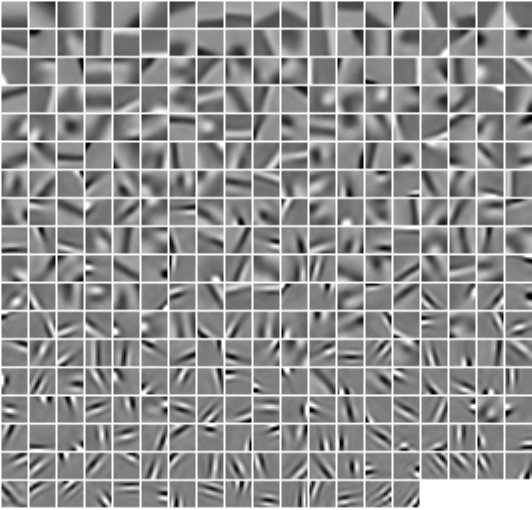
\includegraphics[scale=0.20]{./figures/basisexample.jpg}
        \caption{Sparse basis functions learned from images.}
        \label{fig:basex}   
\end{figure}

These basis vectors are used with activations to represent an image. The activation matrix is best represented in the figure below, where a part of an image uses the activated vectors (non-black) to represent the corresponding image.

\begin{figure}[H]
\centering
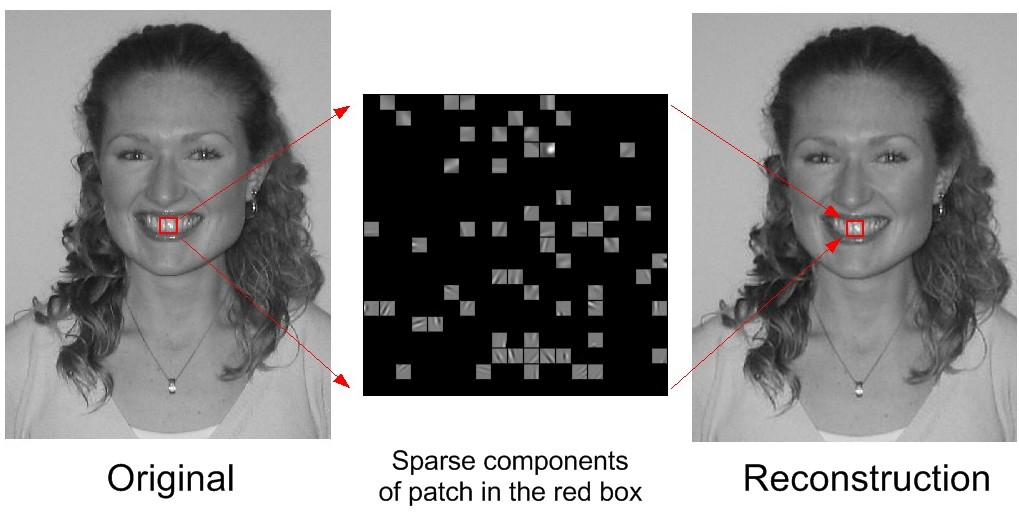
\includegraphics[scale=0.30]{./figures/Sparsejen_black_v2.jpg}
\caption{An image, encoded with the basis functions from figure \ref{fig:basex} and reconstructed in the right plot using certain subsets of activations and basis functions for each patch. The red square represents a patch where we have encoded the activations for some basis functions, shown as the middle plot, to reconstruct the patch of the decoded image to the right. Notice, among the entire set of basis functions, only a fair amount is used and the rest is black indicated that they are not being used, i.e. we have a "sparse" representation of the image. \protect\footnotemark
}
\label{fig:recex}
\end{figure}

\end{ex}
\footnotetext{Peter Foldiak and Dominik Endres ,Scholarpedia, \texttt{http://www.scholarpedia.org/article/Sparse\_coding}, 2008, (accessed 10 June 2015)}
\newpage

\subsubsection{Sparse Coding}

\label{sec:sc}
Sparse Coding is similar to Principal Component Analysis (PCA) in that we want to find a small number of basis functions to represent an input signal as a linear combination presented in equation \ref{eq:lincomb} but with a constraint that the learned basis functions need to be sparse and of a higher dimension than the input data. Here we present the general theory behind Sparse Coding and an example used for signal processing in example \ref{ex:sc} \cite{olshausen}.

\begin{equation}
\mathbf{x} \approx \mathbf{BA}
\label{eq:lincomb}
\end{equation}

Consider a linear system of equations $\mathbf{x} = \sum_{i=1}^ka_i \phi_i$, the vector coefficients $a_i$ are no longer uniquely determined by the input vector $\mathbf{x}$, where $\sum_{i=1}^ka_i = \mathbf{B}$ is an
underdetermined $m\times p$ matrix $(m \ll p)$. $\mathbf{B}$, is called the dictionary or sometimes design matrix. The problem is to estimate the signal $\alpha$, subject to the
constraint that it is sparse. The underlying motivation for sparse
decomposition problems is that even though the observed values are in
high-dimensional ($m$) space, the actual signal is organized in some
lower-dimensional subspace $(k \ll m)$. This implies that $\mathbf{x}$ can be decomposed as a linear combination of only a few $m \times 1$ vectors in $\mathbf{B}$, called atoms \cite{sc}.

Regular PCA allows us to learn a complete set of basis vector while the Sparse Coding wishes to learn an \textbf{over-complete}
basis to recognize patterns and structures inherent in the input data.
Although we now can recognize patterns in the data, we have coefficients of the columns
$\alpha_i$ that are no longer uniquely determined by the input vector
$\mathbf{x} \in \mathbb{R}^2$. This is why we introduce a criterion called
\textbf{sparsity} to resolve the degeneracy introduced by
over-completeness, where sparsity is defined as having few non-zero
components. The definition of the sparse coding cost function on a set of $m$
input vectors is presented in equation \ref{eq:sccost}. In artificial
neural networks, the cost function represents a function to return a number representing how well the neural network performed to map training examples to correct output \cite{olshausen}.

%\begin{equation}
%\mathbf{x} = \mathbf{BA}
%\label{eq:lincomb}
%\end{equation}
%
%Consider a linear system of equations $\mathbf{x} = \mathbf{BA}$, where $\mathbf{B}$ is an
%under-determined $m\times p$ matrix $(m \ll p)$. $\mathbf{B}$, is called the dictionary or the design matrix. The problem is to estimate the signal $\mathbf{A}$, subject to the
%constraint that it is sparse. The underlying motivation for sparse
%decomposition problems is that even though the observed values are in
%high-dimensional ($m$) space, the actual signal is organized in some
%lower-dimensional subspace $(k \ll m)$. This implies that $\mathbf{x}$ can be decomposed as a linear combination of only a few $m \times 1$ vectors in $\mathbf{B}$, called atoms. 
%
%Regular PCA allow us to learn a complete set of basis vector while the Sparse Coding wish to learn a \textbf{over-complete}
%basis to recognize patterns and structures inherent in the input data.
%Although we now can recognize patterns in the data, we have coefficients of the columns
%$\mathbf{B}^(j)$ that are no longer uniquely determined by the input vector
%$\mathbf{x} \in \mathbb{R}^2$. This is why we introduce a criterion called
%\textbf{sparsity} to resolve the degeneracy introduced by
%over-completeness, where sparsity is defined as having few non-zero
%components. The definition of the sparse coding cost function on a set of $m$
%input vectors is presented in equation \ref{eq:sccost}. In artificial
%neural networks, the cost function represents a function to return a number representing how well the neural network performed to map training examples to correct output.

\begin{equation}
\min_{a_i^{(j)},\phi_i}\sum_{j=1}^m
\ \underbrace{\norm{\mathbf{x}^{(j)}-\sum_{i=1}^ka_i^{(j)}\phi_i}^2}_{\text{reconstruction term}}+\underbrace{\lambda \sum_{i=1}^k
S(a_i)^{(j)}}_{\text{sparsity penalty}}
\label{eq:sccost}
\end{equation}

where $S(a_i^{(j)})$ is a sparsity cost function which penalize $a_i$ for being far from zero.
%and $\norm{\mathbf{x}^{(j)}-\sum_{i=1}^ka_i^{(j)}\phi_i}^2 = \sum_{ij} [\mathbf{x}_{ij}-(a \phi)_{ij} ]^2$.
The first term in equation \ref{eq:sccost} is a reconstruction term that forces the algorithm to provide a good representation of $\mathbf{x}$ and the second as a sparsity penalty which force the representation to be sparse, while $\lambda$ is a scale to determine the relative importance between the two contributions. Note that if we are given $S(a_i^{(j)})$, estimation of $\phi_i$ is easy via least squares. In the beginning, we do not have $S(a_i^{(j)})$ however. Yet, many algorithms exist that can solve the objective above with respect to $S(a_i^{(j)})$. 

%Actually, this is how we do inference: we need to solve an optimisation problem if we want to know the h belonging to an unseen $\mathbf{x}$.
% timo banned it

The most direct approach to determine sparsity is through the "$L_0$" norm $S(a_i) = \mathbf{1}(|a_i| > 0 )$, which is non-differentiable and difficult to optimize. The more common choices for sparsity cost penalty $S(a_i)$ are the $L_1$, $S(a_i) = |a_i|_1$ and the log penalty $S(a_i)=\log(1+a^2_i)$. To prevent empirical scaling of $a_i$ and $\phi_i$ to make the sparsity penalty arbitrarily small, we constrain $\norm{\phi}^2$ to be less than some constant $C$. Including the constraint demand we get the full sparse coding cost function \cite{olshausen}

\begin{align}
\begin{split}
\min_{a_i^{(j)},\phi_i} \quad & \sum_{j=1}^m
\norm{\mathbf{x}^{(j)}-\sum_{i=1}^ka_i^{(j)}\phi_i}^2+\lambda \sum_{i=1}^kS(a_i)^{(j)}
\\
\text{subject to} & \quad \norm{\phi_i}^2 \leq C, \forall \ i = 1,\dots,k
\end{split}
\end{align}

Below we present another example of sparse coding but used in a context of signal processing of a one dimensional signal.
\begin{ex}{}
\label{ex:sc}
Say, we have an infinite $1-D$ time-series signal. We can represent this signal in the Fourier domain, where we get a few coefficients representing the whole signal in a different domain.
\begin{equation*}
\mathbf{x} = \sum_{i=1}^k a_i \phi_i \approx \mathbf{x}'
\end{equation*}

We want to find these few coefficients ($a_i$,the basis) of an input signal in the alternative domain and reconstruct your signal with these few coefficients. Once we have found the coefficients, we determine how close is the reconstructed signal to our original input signal by the error. That is to minimize our representation: $|\mathbf{x}- \mathbf{x}'|$.

The least number of basis functions of the input signal that minimize the above error, is the best basis representation of our input signal. We then could use the $L_2$ norm for the error, which is what we are most familiar with and it computes the Euclidean, square difference, between basis functions. Basically, $L_0$ norm looks like a Dirac Delta Function, $L_1$ norm looks like a diamond and $L_2$ norm looks like a circle and are the other types of norms which can be used in this context.

\end{ex}

To end this section we would like to review the difference between Sparse Coding, Autoencoders and Sparse-PCA, as it is somewhat missleading at times.

\begin{itemize}
	\item{Autoencoders do not encourage sparsity in their general form.}
	\item{An autoencoder uses a model for finding the codes, while sparse coding does so by means of optimisation.}
\end{itemize}

Note that Sparse Coding, looks almost the same as Autoencoder as in equation \ref{eq:auto} in section \ref{sec:autoencoders} Autoencoders, once we set $\mathbf{B}=\sigma (\mathbf{A}^T\mathbf{x})$. For natural image data, regularized autoencoders and sparse coding tend to yield very similar $\mathbf{B}$. However, auto encoders are much more efficient and are easily generalized to much more complicated models. E.g. the decoder can be highly nonlinear, e.g. a deep neural network. Therefore, Sparse coding can be seen as a modification of the sparse autoencoder method in which we try to learn the set of features for some data "directly".

In Sparse-PCA one also wants to represent a collection of vectors as a linear combination of basis vectors (a.k.a. principal components). Here the focus, as in traditional PCA, is on choosing a small $n \ll M$ number of basis vectors that together "explain as much variance" as possible, i.e. represent the original data as well as possible. And the sparsity is enforced not on the mapping bases $\rightarrow$data, but on the mapping data$\rightarrow$bases, because the idea is to have PCs that are linear combinations of only small subsets of original features/vectors (to ease the interpretation), as explained in Zou, Hastie, and Tibshirani, 2006 \cite{zou}.

\subsubsection{Non-Negative Sparse Coding}

\label{sec:nnsc}
In standard Sparse Coding, described above, the data is described as a combination of elementary features involving both additive and subtractive interactions. The fact that features can ‘cancel each other out’ using subtraction is contrary to the intuitive notion of combining parts to form a whole \cite{hoyer}. Arguments for non-negative representations come from biological modeling, where such constraints are related to the non-negativity of neural firing rates. These non-negative representations assume that the input data $\mathbf{X}$, the basis $\mathbf{B}$, and the hidden components $\mathbf{A}$ are all non-negative. Since energy consumption is an inherently non-negative quantity, this representation is beneficial is reasonable for modeling energy usage. \\
Non-negative matrix factorization (NMF) can be performed by the minimization of the following objective function:

\begin{equation}
\label{eq:nmf}
C ( \mathbf{A,B} ) = \frac{1}{2} \norm{ \mathbf{X} - \mathbf{BA} }^2
\end{equation}

Here Hoyer \cite{hoyer} take $ \norm{ \mathbf{X} - \mathbf{BA} }^2 = \sum_{ij} [ \mathbf{X}_{ij} - \mathbf{BA}_{ij} ]^2$. Denoting a general matrix norm by

\begin{equation}
\| A \|_{p,q}  =  \left[\sum_{j=1}^n \left( \sum_{i=1}^m |a_{ij}|^p \right)^{q/p}\right]^{1/q}
\end{equation}

Using $p=2,q = 2$ we get the Frobenius norm and we conclude that equation \ref{eq:nmf} is using the Frobenius norm, this is an insurance for later use in the Discriminative Disaggregation via Sparse Coding model \ref{alg:ddsc}.
\[ \|A\|_F^2 =\left(\sqrt{\sum_{i=1}^m\sum_{j=1}^n |a_{ij}|^2}\right)^2 = \sum_{i,j}[a_{ij}]^2\]


\textbf{Definition 1.} Non-negative sparse coding (NNSC) of a non-negative data matrix $\mathbf{X}$ (i.e. $\forall \ i,j \ : \ X_{ij} \geq 0$) is given by the minimization of
\begin{equation}
\label{eq:nnsc}
C ( \mathbf{A,B} ) = \frac{1}{2} \norm{ \mathbf{X} - \mathbf{BA} }^2 + \lambda \sum_{ij} \mathbf{A}_{ij}
\end{equation}
subject under the constraints $\forall \ i,j \ : \ B_{ij} \geq 0, \ A_{ij} \geq 0$ and $\forall \ i \ : \ \| \mathbf{B}_i \| = 1$, where $\mathbf{B}_i$ denotes the i:th column of $\mathbf{B}$. It is also assumed that the constant $\lambda \geq 0$. 
~\\

\pagebreak
\textbf{Theorem 1.} The equation \ref{eq:nmf} is non-increasing under the update rule:
\begin{equation}
\label{eq:update}
\mathbf{A}^{t+1}=\mathbf{A}^t.*(\mathbf{B}^T\mathbf{X})./(\mathbf{B}^T\mathbf{B}\mathbf{A}^t+\lambda)
\end{equation}
where $.*$ and $./$ denote element-wise multiplication and division (respectively), and the addition of the scalar $\lambda$ is done to every element of the matrix  $\mathbf{B}^T\mathbf{B}\mathbf{A}^t$.
~\\

The proof is seen below in \ref{proof:noninc}. As each element of $\mathbf{A}$ is updated by simply multiplying with some non-negative factor, it is guaranteed that the elements of $\mathbf{A}$ stay non-negative under this update rule. As long as the initial values of $\mathbf{A}$ are all chosen strictly positive, iteration of this update rule is in practice guaranteed to reach the global minimum to any required precision.

\begin{proof2}{Proof of Theorem 1}
To prove Theorem 1, first note that the equation \ref{eq:nnsc} in definition 1 is separable in the columns of $\mathbf{A}$ so that each column can be optimized without considering the others. We may thus consider the problem for the case of a single column, denoted s. The corresponding column of $\mathbf{X}$ is denoted $x$, giving the objective
\begin{equation}
F(\mathbf{a}) = \frac{1}{2}\norm{\mathbf{X}-\mathbf{B}\mathbf{a}}^2 + \lambda \sum_i a_i
\end{equation}
We need an iliary function $G(\mathbf{a},\mathbf{a}^t)$ with the properties that $G(\mathbf{a},\mathbf{a}) = F(\mathbf{a})$ and $G(\mathbf{a},\mathbf{a}^t) \geq F(\mathbf{a})$. We will then show that the multiplicative update rule corresponds to setting, at each iteration, the new state vector to the values that minimize the auxiliary function:
\begin{equation}
\mathbf{a}^{t+1} = \arg\!\min_{a} G(\mathbf{a},\mathbf{a}^t).
\end{equation}
This is guaranteed not to increase the objective function $F$, as
\begin{equation}
\label{eq:proof}
F(\mathbf{a}^{t+1}) \leq G(\mathbf{a}^{t+1},\mathbf{a}^t) \leq G(\mathbf{a}^t,\mathbf{a}^t) = F(\mathbf{a}^t).
\end{equation}
We define the function $G$ as
\begin{equation}
G(\mathbf{a},\mathbf{a}^t) = F(\mathbf{a}^t) + (\mathbf{a}-\mathbf{a}^t)^T \nabla F(\mathbf{a}^t) + \frac{1}{2} (\mathbf{a}-\mathbf{a}^t)^T\mathbf{K}(\mathbf{a}^t)(\mathbf{a}-\mathbf{a}^t)
\end{equation}
where the diagonal matrix $\mathbf{K}(\mathbf{a}^t)$ is defined by elementwise division as
\begin{equation}
K_{ij}(\mathbf{a}^t) = \delta_{ij}\frac{(\mathbf{B}^T\mathbf{B}\mathbf{a}^t)_i+\lambda}{\mathbf{a}^t_i},
\end{equation}
where $i$ denotes the $i$:th column. Inserting $\mathbf{a}$ in function $G$ we get the result from equation \ref{eq:proof}, $G(\mathbf{a},\mathbf{a}) = F(\mathbf{a})$. Writing out
\begin{equation}
F(\mathbf{a}) = F(\mathbf{a}^t) + (\mathbf{a}-\mathbf{a}^t)^T \nabla F(\mathbf{a}^t)+\frac{1}{2}(\mathbf{a}-\mathbf{a}^t)^T(\mathbf{B}^T\mathbf{B})(\mathbf{a}-\mathbf{a}^t),
\end{equation}
we see that the second property, $G(\mathbf{a},\mathbf{a}') \geq F(\mathbf{a}),$ is satisfied if
\begin{equation}
0 \leq (\mathbf{a}-\mathbf{a}^t)^T[\mathbf{K}(\mathbf{a}^t) - \mathbf{B}^T\mathbf{B}](\mathbf{a}-\mathbf{a}^t).
\end{equation}
Hoyer proved this positive semidefiniteness for the case of $\lambda \geq 0$ \cite{hoyer}. He concludes that as a non-negative diagonal matrix is positive semidefinite, and the sum of two positive semidefinite matrices is also positive semidefinite, the proof for $\lambda = 0$, in his paper also holds for $\lambda \geq 0$.
It remains to be shown that the update rule in equation \ref{eq:update} selects the minimum of $G$. This minimum is easily found by taking the gradient and equating it to zero:
\begin{equation}
\nabla_\mathbf{a} G(\mathbf{a},\mathbf{a}) = \mathbf{B}^T(\mathbf{B}\mathbf{a}^t-\mathbf{x}) + \lambda\mathbf{c} + \mathbf{K}(\mathbf{s}^t)(\mathbf{a}-\mathbf{a}^t)=0,
\end{equation}
where $\mathbf{c}$ is a vector with all ones. Solving for $\mathbf{a}$, this gives
\begin{align}
\mathbf{a} & = \mathbf{a}^t - \mathbf{K}^{-1}(\mathbf{a}^t)(\mathbf{B}^t\mathbf{B}\mathbf{a}^t-\mathbf{B}^T\mathbf{x}+\lambda \mathbf{c}) \\
& = \mathbf{a}^t-(\mathbf{a}^t./(\mathbf{B}^T\mathbf{B}\mathbf{a}^t+\lambda\mathbf{c})).* (\mathbf{B}^T\mathbf{B}\mathbf{a}^t - \mathbf{B}^T\mathbf{x}+\lambda \mathbf{c}) \\
& = \mathbf{a}^t.\times (\mathbf{B}^T\mathbf{x}./(\mathbf{B}^T\mathbf{B}\mathbf{a}^t+\lambda\mathbf{c}))
\end{align}
which is the desired update rule \ref{eq:update}.
\label{proof:noninc}
\end{proof2}


%\subsubsection{Tranformation Algorithms and variations for sparse approximation}
%%
%\label{sec:regularization}
%\subsubsection{Ridge Regression}
%
%A famous method of regularization called Tikhonov regularization, in statistics this method is known as ridge regression, an algorithm for non-linear least-squares problems. When x is non-existent, we call it an ill-posed problem such as below
%
%\begin{equation}
%A\mathbf{x}=\mathbf{b},
%\end{equation}
%
%a standard approach to the problem is ordinary least squares, which often leads to an underdetermined system of equations. Real-world problems often operate as a low-pass filter, meaning that the direction of the mapping where $A$ maps $\mathbf{x}$ to $\mathbf{b}$. By the inverse-mapping, we operate as a high-pass filter, which is often the case in mathematical formulations, it has an undesirable tendency of amplifying noise. \cite{ill-posed} Ordinary least squares (OLS) nullifies every element of the reconstructed elements of $\mathbf{x}$, that is in the null-space of $A$. The ridge regression uses the $l_2$-norm as a means of regression to the residuals and can be mathematically written as the following formulation
%\begin{equation}
%\label{eq:ridge}
%\beta^{ridge} = \arg \! \operatorname*{\min}_\beta \sum_{i=1}^n (\mathbf{y}_i - ( \beta_0 + \beta^T \mathbf{x}_i))^2 + \lambda \norm{\beta}^2_2
%\end{equation}
%There are other techniques which are based on the assumption that the $l_2$-norm does not capture the features to the respective dimensions and therefore "LASSO" has been used as a means of using the $l_1$-norm instead.
%
%\subsubsection{LASSO}
%
%"LASSO" In the context of regression and statistics, is fittingly being used as a metaphor of $L_1$ constraint applied to linear model. Coincidently, LASSO is also the initials for Least Absolute Shrinkage and Selection Operator. LASSO minimizes the residual sum of squares subject to the sum of the absolute value of the coefficients being less than a constant. LASSO not only helps to improve the prediction accuracy when dealing with multicolinearity data, but also carries several nice properties such as interpretability and numerical stability. Because of the nature of this constraint it tends to produce some coefficients that are exactly 0 and hence gives interpretable models \cite{lasso}. In a Bayesian context, this is equivalent to placing a zero-mean Laplace prior distribution on the parameter vector \cite{bayes_lasso}. The optimization problem may be solved using quadratic programming or more general convex optimization methods. The formulation of LASSO regression can mathematically be written as
%
%\begin{equation}
%\label{eq:lasso}
%\beta^{lasso} = \arg \! \operatorname*{\min}_\beta \sum_{i=1}^n (\mathbf{y}_i - ( \beta_0 + \beta^T \mathbf{x}_i))^2 + \lambda \norm{\beta}_1
%\end{equation}
%
%The difference between LASSO and ridge regression is that the penalty is increased and all parameters remain non-zero while still being reduced, using ridge regression. While increasing the penalty using LASSO will cause more and more of the parameters to be driven to zero. This makes LASSO an advantage for practical and model evaluation reasoning as we have to deal with less parameters to the model. As a result, LASSO selects more relevant features and discards the others, whereas ridge regression never fully discards any features. \cite{bayes_lasso}
%
%\subsubsection{Gradient Descent}
%
%The gradient descent method gives a way to find a local minimum of a given general function. We initialize the algorithm by a guess to the solution and compute the gradient for the function at the initial point. Next, we start the process of stepping through the negative direction of the gradient and repeat the process until the algorithm has converged at which the gradient is zero or until we reach a point at which we believe that there is no local minimum. The algorithm is called a first-order algorithm as it only takes the first derivative of the function into account.
%
%Here we will walk through the process of a gradient descent algorithm for finding the solution to the minimum of some function $f(x)$. Initializing with some initial value $x_0$ for $x$, we can change its value proportional to the dimension of x: with only one dimension; we can make it higher or lower. The best direction at $x_0$ to minimize $f$, we take the gradient $\nabla f$ along every dimension of $x$. Intuitively, the gradient will give the curve at that which $x$ will point to an increase in the function. Therefore we change $x$ in the opposite direction to lower the function value:
%\begin{equation}
%x_{k+1} = x_k - \lambda \nabla f(x_k)
%\end{equation}
%where $\lambda$ represents the stepsize in the discretization of the function we represent. This can be a fixed value or change depending on which implementation one decides to chose. Often $\lambda>0$ is a small number that forces the algorithm to make small jumps, even for the most minimal $\lambda$ it has been shown to converge to a minimum. As a result, the algorithm will be stable and its optimal value depends on the function, given stable conditions (and a certain choice of $\lambda$), it is guaranteed that $f(x_{k+1}) \leq f(x_k)$ \cite{gradient}.
%
%\subsubsection{Coordinate Descent}
%
%Instead of relying on the gradient of a function, one approach called the coordinate descent can minimize a function by minimizing it along one direction at a time. By the given regression model we can minimize the function $f(x)$.
%\begin{equation}
%y = X \theta,
%\end{equation}
% the function to minimise for a least squares regression is 
% \begin{equation}
% f(\theta) = | y- X \theta |^2.
% \end{equation}
% Minimising over $\theta$ is achieved by 
% \begin{equation}
% 0 = X_{i}^\top (X \theta - y) = X_{i}^\top (X_i \theta_i + X_{-i} \theta_{-i} -y).
% \end{equation}
% So the next step in the coordinate descent update is
% \begin{equation}
% \theta_{i} = \frac{X_{i}^\top(y- X_{-i}\theta_{-i})}{X_{i}^\top X_{i}}.
% \end{equation}
%Regardless the learning rate of the gradient descent procedure (which could indeed speed up convergence), the comparison between the two is fair at least in terms of complexity.
%Coordinate descent needs to perform $O(n)$ operations for each coordinate update (n operations to compute residuals $r = (y- X_{-i}\theta_{-i})$ and n to compute $X_{i}^\top r$ . Each cycle of this type is performed p times, where p is the number of covariates.
%Gradient descent performs the same number of operations $O(np)$.
%
